%
% COMMENT
%
\begin{comment}

\subsection{Object navigation}\label{sec:object-navigation}

After all the objects have been spotted, an intelligent route to pick up these is needed. The \projname{} uses the nearest neighbour search (NNS) algorithm to pick up the objects. The algorithm used is shown in \lstref{lst:objectnavigation1} and \lstref{lst:objectnavigation2}. The algorithm looks at the position and distance to all objects, and from the position of the \projname{}, decides what object to pick up first. From the position of the first collected object it decides, from this position, the shortest distance to the next object, and so forth until all the objects are included in the route. 


\subsubsection*{Object navigation --- concept} \label{sec:objnav-concept}
The algorithm uses trigonometry to select the next object, using the object positions observed from the starting positions. The degrees the \projname{} must turn, in order to get to the same heading as the object, is saved as instructions, along with the distance. These instructions must then be followed after the route has been calculated. \figref{fig:object_navigation_first} shows a situation where all the objects have been spotted, and now the \projname{} must decide which object that should be collected first. At this point the shortest object is easy to conclude, as the distance to all objects, from the starting position, is already known. The shortest distance overall is found, and the object associated to this is remembered, and marked as collected, to remove this from consideration when finding the next objects. Then the objects angle and the distance is saved into the instructions array. Another set of instructions is used to ensure that the \projname{} is pointing back, at the starting position. This is used to ease the calculations of the next objects. 

\begin{figure}[H]
     \center{\frame{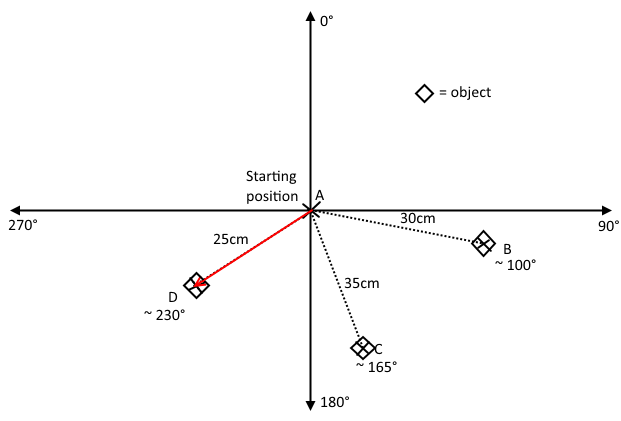
\includegraphics[width=\textwidth]
     {graphics/objectnavigationfirst.png}}}
     \caption{\label{fig:object_navigation_first} First object to be collected.}
\end{figure}

Now that the first object has been scheduled to be collected, the calculations uses trigonometry to find the shortest distance to the next object, and the angles that needs to be turned to face the starting position again. To increase the understanding, the state of the world is represented in \figref{fig:object_navigation_iteration}, where the actions to collect the first object has been applied and reflected in the figure. From this point, the distance to the remaining objects is calculated, using the formula:

\begin{equation}
a = \sqrt{ b^2 + c^2 - 2*b*c*cos(A) } \label{equation:a}
\end{equation}

But for this, the A angle is needed. This is calculated from the spotted angles during the search. The formula for calculating A is:

\begin{equation}
A = (Object~currently~at~spotted~angle) - (Object~closest~spotted~angle) \label{equation:AAngle}
\end{equation}

With the same method as the first object, the object with the shortest distance, from the current object, is found and saves the object number. Now the heading to the closest object must be calculated, and this is the angle calculated by the formula:

\begin{equation}
B = cos^{-1}((a^2 + c^2 - b^2)/(2*a*c)) \label{equation:B}
\end{equation}

This provides the angle that must be turned in order to face the next object. In \figref{fig:object_navigation_iteration} the \projname{} is pointed towards the starting position, and the angle that must be turned is calculated from equation \ref{equation:B}. The current heading added with the angle provides the heading to the next object. This angle is added to the instructions along with the distance. Then the final angle of the triangle is calculated, which is used to turn the \projname{} at the starting position again. The final angle is calculated with the formula:

\begin{equation}
C = 180 - A - B \label{equation:C}
\end{equation}

In order to point the \projname{} at the starting position again, the current heading is subtracted with (180 - C), where C is found by equation \ref{equation:C}. This process has provided the route to the next object, and the instructions to turn the \projname{} back, facing the starting position. The second step is executed for the remaining objects that were spotted. 

\begin{figure}[H]
     \center{\frame{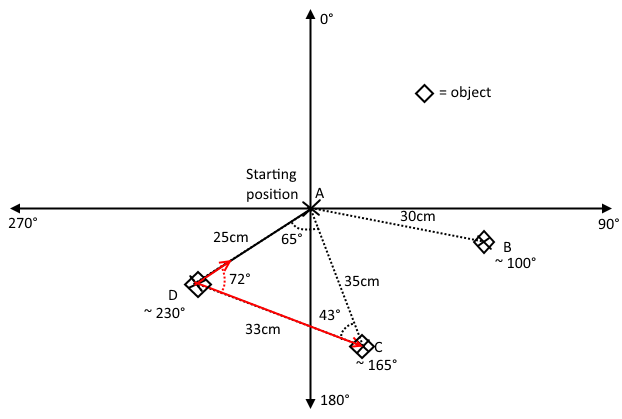
\includegraphics[width=\textwidth]
     {graphics/objectnavigationiteration.png}}}
     \caption{\label{fig:object_navigation_iteration} Iteration of objects to be collected.}
\end{figure}



%
% COMMENT
%
%\begin{comment}
\subsubsection*{Object navigation - implemented} \label{sec:objnav-implemented}

\lstref{lst:objectnavigation1} and \lstref{lst:objectnavigation2} shows the algorithm, as tried to implemented in the \projname{}. It practically works the same way as the concept, but with a few adjustments to make it work. An important little workaround is the boolean \emph{flipped} variable. This is used to decide to which direction, the \projname{} should turn, in order to get to the next object. The problem with choosing the direction is sketched in \figref{fig:choosingdirection}, to help understanding. The difference in angles is calculated, from the object where the \projname{} is currently at. Then angle is checked using the \emph{CalculateValidAngle} function, that ensures that the value is within the possible values (0 - 359). If the difference in angle is bigger than 180, then the flipped variable is set to true, meaning that the turning direction is left, else turn to the right. The \emph{flipped divider}, from \figref{fig:choosingdirection}, shows to which side the \projname{} should turn, depending on which side the object is located. Depending on which side the object is located, different measures to find the angle is used, as shown on in \figref{fig:choosingdirection} This provides us with the correct angle, that should be turned to face the next object. 

\begin{figure}[H]
     \center{\frame{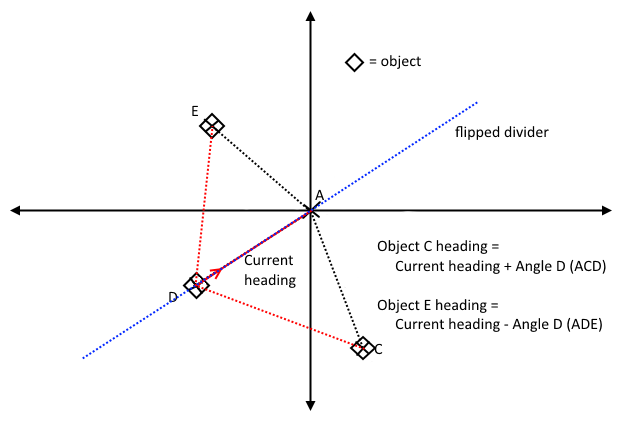
\includegraphics[width=\textwidth]
     {graphics/objnavchoosingdirection.png}}}
     \caption{\label{fig:choosingdirection} Choosing the direction.}
\end{figure}

The algorithm used a boolean array to control which object it has collected, ensuring that the object is removed from the remaining objects, as the \projname{} should only get to each object once. 

The first part of the algorithm can be seen in \lstref{lst:objectnavigation1}. This part shows the initialisation of variables and the input parameters. At line 19, the helper function \emph{FindClosestObjects} is used to find the closest object. Then the case for the first object is shown, where no trigonometry is needed to calculate, as this is from the starting position, knowledge about angle and distance is known from the sensors. 

\begin{lstlisting}[caption= Object navigation start and for the first object, label=lst:objectnavigation1]
void ObjectNavigation(OBJECT objects[], int objectsFound, OBJECT instructions[], OBJECT turnToStartInstructions[])
{
	int addedToRoute = 0;
	int previousObjectNumber = 0;
	int closestObjectNumber = 0;
	S16 currentHeading = compass.getHeading(); 
	bool hasBeenAdded[objectsFound];
	bool flipped = false; 
	
	for (int j = 0; j <= objectsFound; j++)
	{
		flipped = false; 
		closestObjectNumber = findClosestObjects(objects, objectsFound, addedToRoute, previousObjectNumber,  hasBeenAdded);
		
		if (j == 0)
		{
			instructions[j].angle = objects[closestObjectNumber].angle;
			currentHeading = objects[closestObjectNumber].angle;
			instructions[j].distance = objects[closestObjectNumber].distance;
			hasBeenAdded[closestObjectNumber] = true;
			
			previousObjectNumber = closestObjectNumber;
			turnToStartInstructions[j].angle = CalculateValidAngle(currentHeading, 180);
			currentHeading = turnToStartInstructions[j].angle;
			addedToRoute++;
		}
\end{lstlisting}

\lstref{lst:objectnavigation2} shows the case for the n'th object. The difference here is the use of trigonometry to calculate the next angle to turn and distance to travel. Mathematical concepts presented in \secref{sec:objnav-concept} is used to calculate the angles and distances. 

\begin{lstlisting}[caption= Object navigation n'th object, label=lst:objectnavigation2]
		else if (j > 0)
		{
			int b = objects[closestObjectNumber].distance;	
			int c = objects[previousObjectNumber].distance;
			int aAngle = CalculateValidAngle(objects[previousObjectNumber].angle, -objects[closestObjectNumber].angle);
			if (180 < aAngle && aAngle <= 359)
			{
				flipped = true;
			}
			int a = static_cast<int>(sqrt(pow(b, 2)+pow(c, 2)-2*b*c*cos((aAngle*PI)/180)));
			int bAngle = static_cast<int>(acos((pow(a, 2)+pow(c, 2)-pow(b, 2))/(2*a*c)) * 180 / PI);
			int cAngle = ((180 - aAngle) - bAngle);

			instructions[j].angle = (flipped == false) ? (currentHeading+bAngle) : (currentHeading-bAngle);
			instructions[j].distance = a;
			hasBeenAdded[closestObjectNumber] = true; 
			previousObjectNumber = closestObjectNumber;
			turnToStartInstructions[j].angle = (flipped == false) ? CalculateValidAngle(currentHeading, (180-cAngle)) : CalculateValidAngle(currentHeading, -(180-cAngle));
			currentHeading = turnToStartInstructions[j].angle;
			addedToRoute++;
		}
	}
}
\end{lstlisting}


The algorithm uses a function to help find the closest object. This is used to divide the task to increase readability. The \emph{FindClosestObject}, seen in \lstref{lst:findclosestobject}, takes all the objects as input, an array to check which object has been added and knowledge about the last object that was chosen. From this, it checks the objects, those that has not already been added, from the last objects location. The last objects location is the starting position for the first object. The distance to all the other remaining objects is then calculated and the object closest is chosen and returned. 

\begin{lstlisting}[caption= Function findClosestObject, label=lst:findclosestobject]
int FindClosestObjects(OBJECT objects[], int objectsFound, int addedToRoute, int previousObjectNumber, bool hasBeenAdded[])
{
	int closestObjectNumber = -1; 
	int tempDistance = 2000; 
	
	for (int i = 0; i <= objectsFound; i++)
	{
		if (addedToRoute == 0)
		{
			if (objects[i].distance < tempDistance)
			{
				tempDistance = objects[i].distance;
				closestObjectNumber = i;
			}
		}
		
		else if (addedToRoute > 0 && hasBeenAdded[i] == false)
		{
			int b = objects[i].distance;
			int c = objects[previousObjectNumber].distance;
			int aAngle = objects[previousObjectNumber].angle - objects[i].angle;
			if ( aAngle < 0 )
			{
				aAngle = -aAngle;
			}
			int a = static_cast<int>(sqrt(pow(b, 2)-pow(c, 2)-2*b*c*cos((aAngle*PI)/180)));
			
			if ( a < tempDistance )
			{
				tempDistance = a;
				closestObjectNumber = i;
			}
		}
	}
	return closestObjectNumber;
}
\end{lstlisting}

Despite several tests and number tweaking within the algorithm, the problems with the ultrasonic sensor, see \secref{sec:ultrasonic_sensor}, were too severe to get the initial search to work. The sensor were not able to spot the right amount of objects and the precision of the objects were not correct, which resulted in a calculated route that would not hit the objects. It was therefore decided to use the next-in-view algorithm as described in the sixth iteration in \secref{sec:imp-procedure}.
\end{comment}
%
% COMMENT
%